%% ----------------------------------------------------------------
%% Thesis.tex -- MAIN FILE
%% ---------------------------------------------------------------- 

% Set up the document
\documentclass[a4paper, 12pt, oneside,spanish]{Thesis} 
\graphicspath{{Imagenes/}}  

\usepackage[spanish]{babel}
\usepackage[square, numbers, comma, sort&compress]{natbib}  
\usepackage{verbatim}  
\usepackage{vector}  
\usepackage[latin1]{inputenc}
\usepackage[nottoc] {tocbibind}
\hypersetup{urlcolor=blue, colorlinks=true}  

%% ----------------------------------------------------------------
\begin{document}
\frontmatter      

\title  {
Confidencialidad de Datos en Aplicaciones Android
}
\addresses  {\groupname\\\deptname\\\univname} 
\authors  {\texorpdfstring
            {\href{gastaldidiego93@gmail.com}{Diego Gastaldi}}
            {Diego Gastaldi}
            }
\supervisor     {\texorpdfstring
            {\href{pancho@dc.exa.unrc.edu.ar }{Francisco Bavera}}
            {Francisco Bavera}
            }
\date       {\today}
\keywords   {}

\maketitle
%% ----------------------------------------------------------------

\setstretch{1.3}  

\fancyhead{}  
\rhead{\thepage} 
\lhead{}  

\pagestyle{fancy}  

\clearpage  

%% ----------------------------------------------------------------

% The Abstract Page
\addtotoc{Resumen} 
\abstract{
\addtocontents{toc}{\vspace{1em}}  % Add a gap in the Contents, for aesthetics

Aplicaciones {\tt Android}, tanto maliciosas y mal intencionadas como programadas descuidadamente o mal, pueden filtrar informaci�n importante 
de los usuarios. Para detectar estas filtraciones de informaci�n se pueden analizar las aplicaciones con distintos enfoques. Esta trabajo 
presenta el desarrollo de una herramienta basada en an�lisis est�tico para detectar filtraciones de informaci�n. 
Combinando y extendiendo diferentes trabajos previos como {\tt DidFail} \cite{Didfail}, {\tt Flowdroid} \cite{Flowdroid}, {\tt Epicc} \cite{Epicc}, 
{\tt Soot} \cite{Soot}, entre otros se obtiene una herramienta que 
permite realizar el an�lisis sobre un conjunto de aplicaciones, donde se identifican las posibles comunicaciones inter-aplicaci�n 
(comunicaci�n entre componentes de diferentes aplicaciones) e intra-aplicaci�n (comunicaciones entre componentes de una misma aplicaci�n), 
con el fin de detectar filtraciones de informaci�n confidencial. \par

El usuario puede crear un jerarqu�a de niveles de seguridad y asign�rselas a diferentes informaciones que pueden fluir 
entre las distintas aplicaciones. La herramienta permite configurar una pol�tica de seguridad multinivel.
Junto con ellas, el usuario puede brindar excepciones, permitiendo a flujos que violen los niveles de 
seguridad no ser considerado peligroso. Este �ltimo punto, permite flexibilidad y que la herramienta pueda ser utilizada en  aplicaciones reales.\par

La herramienta genera informaci�n del flujo de los datos en el programa, luego, con la informaci�n obtenida se analiza  
que el flujo de la informaci�n no viole la pol�tica de seguridad asignada por el usuario (que se respeete la jerarqu�a de niveles de seguridad de los datos). 
Este �ltimo paso se realiza aplicando una implementaci�n del algoritmo de {\it Jacob Rehof} y {\it Torben Mogensen} \cite{JacobRehofTorbenMogensen}. \par

Este informe describe el m�todo de an�lisis, implementaci�n y resultados experimentales de la herramienta obtenida. \par
}

\clearpage  

%% ----------------------------------------------------------------

\pagestyle{fancy}  

%% ----------------------------------------------------------------
\lhead{\emph{Contents}}  
\tableofcontents  

%% ----------------------------------------------------------------
\mainmatter
\pagestyle{fancy} 

 \lhead{\emph{Introducci�n}}
\chapter{Introducci�n}

Este proyecto consiste en desarrollar una herramienta que lleve a cabo el an�lisis est�tico de programas Android, el cual toma como entrada un conjunto de aplicaciones destinadas al sistema operativo Android, luego las decompila, es decir, obtiene su c�digo en alg�n lenguaje espec�fico como puede ser Java o un lenguaje intermedio para as�, poder indagar sobre el flujo de la informaci�n del dispositivo y comprobar si estas aplicaciones tiene un comportamiento malicioso. \par
Como antecedentes de trabajos relacionados con esta idea podemos nombrar DidFail \cite{Didfail}, Flowdroid \cite{Flowdroid}, DroidSafe \cite{DroidSafe}, PScout \cite{PScout}.

\section{Motivaci�n}

La idea surge debido a la deficiencia que tienen los repositorios de aplicaciones Android, ya que, a pesar de que brindan una manera autom�tica, de costo m�nimo, para resolver la distribuci�n o sustituci�n de c�digo para enormes cantidades de destinatarios, esta t�cnica tambi�n entra�a graves riesgos, ya que el software de los repositorios puede comprometer la confidencialidad y/o integridad de los datos de sus numerosos destinatarios, tanto por fallas de programaci�n, como por intenciones maliciosas. Este problema no es nuevo, ni exclusivo de Android, por lo que la b�squeda de soluciones para este problema ha dado origen a activas l�neas de investigaci�n \cite{InformationFlow}. \par
Un ejemplo de la explotaci�n de estas deficiencia se da cuando un usuario de un dispositivo (smartphone, tablet, etc.) instala un juego para Android que filtra toda la lista de contactos del usuario (obteniendo previamente permiso para hacerlo) a una empresa de marketing mediante el env�o de los contactos a otra aplicaci�n con los permisos necesarios para acceder a internet, llev�ndose a cabo la fuga de informaci�n no controlada por el sistema. \par
El problema de la integridad de la informaci�n manipulada por aplicaciones Android es de gran importancia, dado el intenso uso de esta plataforma. Pero, es muy dif�cil y costoso realizar las pruebas y la depuraci�n para garantizar la inexistencia de dicho problema. Por ello, es necesario contar con t�cnicas y herramientas autom�ticas que verifiquen est�ticamente estas propiedades.\par
La aplicaci�n de an�lisis est�ticos inter e intraprocedural que permitan determinar el flujo de la informaci�n permitir� garantizar la confidencialidad e integridad de la informaci�n manipulada por programas Android. La construcci�n de un prototipo podr� clarificar la viabilidad, eficiencia y eficacia del uso de an�lisis est�tico para la verificaci�n de confidencialidad e integridad de la informaci�n.\par


\section{Contribuci�n}

La herramienta desarrollada a�ade a las funcionalidad que ya pose�an los trabajos previos ya mencionados, la posibilidad de asignarle niveles de seguridad a cada m�todos conocido que obtiene informaci�n del usuario y a cada m�todo que permite enviar dicha informaci�n a, por ejemplo, otra aplicaci�n o internet. Para dichos niveles se requiere previamente un orden parcial que los relaciona, para as� poder comprobar si la informaci�n fluye de acuerdo a la jerarqu�a de niveles dada o se produce una violaci�n. \par
Tanto los niveles asignados a cada m�todo como los flujos que deben ser ignorados (excepciones) pueden ser proporcionado por el usuario de dos maneras diferentes: mediante el uso de una interfaz gr�fica o mediante archivos de configuraci�n. \par
Tambi�n, se brinda un archivo de configuraci�n para el establecimiento de la jerarqu�a que relaciona los niveles de seguridad. �sta debe cumplir con ciertos requisitos que se mencionar�n a lo largo del informe.\par
En cuanto a los resultados, se informa del flujo que produce la violaci�n, en caso que exista, o de la ausencia de estos en caso contrario. Dichos resultados pueden verse de la misma manera que las entradas al sistema, es decir, de manera gr�fica o guardado en un archivo.\par
Adem�s, el usuario tiene la posibilidad de no proveer niveles a los m�todos que crea conveniente, permitiendo a la herramienta el c�lculo de un nivel adecuado para evitar problemas de seguridad en caso de ser posible. Estos niveles calculados autom�ticamente se incluyen a los resultados del an�lisis.\par
Por otro lado, se realizaron unas modificaciones en los scripts de Didfail \cite{Didfail} para realizar los an�lisis individuales de las aplicaciones de manera concurrente, y se agregaron otros scripts para los casos en que las aplicaciones ya fueron analizadas individualmente y solo se pretende probar nuevas asignaciones de niveles de seguridad, ya que la primer parte es la m�s costosa en cuanto a tiempos y recursos que utiliza.\par

\section{Estructura del Informe}

El resto del informe est� organizada como sigue: El cap�tulo 2 provee una introducci�n a los concepto importantes como es el an�lisis est�tico, Android (conceptos relacionados con el tema) y un resumen de las herramientas previamente desarrollada que se utilizaron, y adem�s, se presenta un ejemplo motivador. El cap�tulo 3 describe en detalle el aporte provisto por este trabajo, y en el cap�tulo 4 se describe la implementaci�n del mismo. En cuanto al capitulo 5, contiene un ejemplo del uso del analizador juntos con los resultados obtenidos. Se discuten las limitaciones del an�lisis en el cap�tulo 6, y las conclusiones a las que se llegaron en el cap�tulo 7. \par
 
 
 \lhead{\emph{Conocimientos Previos}}
\graphicspath{{Imagenes/}} 

\chapter{Conocimientos Previos}

\section{An�lisis Est�tico}

El an�lisis est�tico es un m�todo de an�lisis en el cual el c�digo fuente es analizado sin ser ejecutado. Como contrapunto, el an�lisis din�mico involucra el estudio  del comportamiento de las aplicaciones a trav�s de la ejecuci�n de las mismas en un ambiente determinado (los dispositivos android en nuestro caso).\par
El an�lisis est�tico permite examinar todas las posibles ejecuciones de un programa. Esto es especialmente valioso en el an�lisis de la seguridad, ya que los ataques suelen explotar aplicaciones de maneras imprevistas y no probados. Sin embargo, predecir el comportamiento del programa sin ejecutar no es un problema trivial. Al reducir al problema de la parada (halt), es posible demostrar que la b�squeda de todas las maneras posibles de ejecutar cualquier programa no trivial arbitrario es un problema indecidible. Sin embargo, el an�lisis est�tico puede proporcionar resultados �tiles mediante la aproximaci�n de algunas facetas de la ejecuci�n real de un programa \cite{AbsInt}.\par
Una de las t�cnicas de an�lisis est�tico lleva a cabo el an�lisis del flujo de datos (data flow). El taint analysis es un tipo especial de an�lisis de flujo de datos que realiza el seguimiento de datos a lo largo del camino de la ejecuci�n del programa. En esta t�cnica, los datos sensibles son marcados con una mancha en la fuente u origen, y se propaga a trav�s de todas las rutas de ejecuci�n del programa. La presencia de este mancha en los sink o destinos predefinidos se utiliza para establecer un flujo entre la fuente y el sink. Este flujo puede ser utilizado para detectar las fugas de datos sensibles desde la fuente a diferentes destinos. Donde, si adem�s, se agregan niveles tanto a los source (fuentes) como a los sinks, se pueden detectar que si informaci�n importante o privada puede estar llegando a lugares p�blicos o no deseados.\par

\section{Information Flow}

La protecci�n de la confidencialidad de la informaci�n manipulada por los sistemas de computaci�n es un problema de larga data, siendo cada vez m�s importante. Las pr�cticas de seguridad est�ndares previas al surgimiento de estudios sobre information-flow \cite{InformationFlow} no ofrec�an garant�as sustanciales de que el comportamiento de extremo a extremo de un sistema inform�tico satisface las pol�ticas de seguridad importantes como la confidencialidad. Una pol�tica de confidencialidad de extremo a extremo podr�a afirmar que los datos de entrada secretas no pueden deducirse por un atacante a trav�s de observaciones sobre salida del sistema; esta pol�tica regula el flujo de la informaci�n.\par
Los mecanismos de seguridad convencionales, tales como el control de acceso y cifrado no se refieren directamente a la aplicaci�n de las pol�ticas de flujo de informaci�n. Analizar las caracter�sticas de confidencialidad de un sistema inform�tico es dif�cil, ya que estos puede incluir errores de implementaci�n y dise�o y, adem�s, como los sistemas inform�ticos modernos com�nmente incorporan hosts o c�digo que no son de confianza, posiblemente maliciosos, hace que la garant�a de confidencialidad sea a�n m�s dif�cil. \par 
Una forma est�ndar para proteger los datos confidenciales es el control de acceso: se requiere alg�n privilegio con el fin de acceder a los archivos u objetos que contienen el datos confidenciales. El problema aqu� es que las verificaciones de control de acceso imponen restricciones a la divulgaci�n de informaci�n, pero no de su propagaci�n. Una vez que la informaci�n es liberado de su contenedor, el programa que accede a ella puede, por error o malicia, inadecuadamente transmitir la informaci�n en alguna forma. No es realista suponer que todos los programas en un sistema de computaci�n grande son dignos de confianza; Por otro lado, los mecanismos de seguridad tales como la verificaci�n de firmas y escaneo de antivirus no garantizan que se mantenga la confidencialidad por el programa revisado. \par
Para asegurar que la informaci�n se utiliza s�lo de acuerdo con las pol�ticas de confidencialidad pertinentes, es necesario analizar c�mo fluye la informaci�n dentro del programa. La creencia de que un sistema es seguro con respecto a la confidencialidad debe surgir de un an�lisis riguroso que demuestre que el sistema en su conjunto hace cumplir las pol�ticas de confidencialidad de sus usuarios. Este an�lisis debe demostrar que la informaci�n controlada por una pol�tica de confidencialidad no puede fluir a un lugar donde se viola esa pol�tica, la Figura 1 muestra un ejemplo b�sico indicando un flujo permitido y uno que no lo es (que viola las pol�ticas de seguridad). Las pol�ticas de confidencialidad que deseamos cumplir son, por lo tanto, las pol�ticas de flujo de informaci�n y los mecanismos que las hacen cumplir son los controles de flujo de informaci�n. Esto di� lugar a un nuevo enfoque: el uso de t�cnicas de lenguajes de programaci�n para especificar y hacer cumplir las pol�ticas de flujo de informaci�n.\par

\begin{center}
 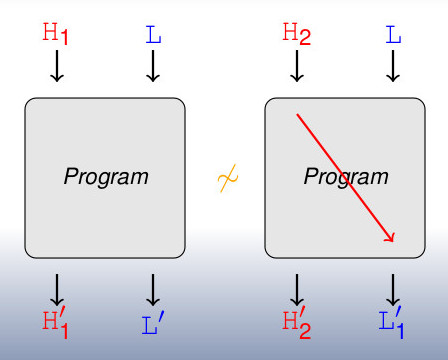
\includegraphics[scale=0.5]{Figura1} \par
 Figura 1: Flujos permitidos y no permitidos.
 \end{center}

El an�lisis de confidencialidad e integridad para lenguajes de bajo nivel (assembly, bytecode) \cite{JavaBytecodeVerif, InformFlowForLowLevel, VerConfPolForMobCod, TypAssLangConf, PreStatAna} a�n tiene un menor desarrollo que el alcanzado para lenguajes de alto nivel (Java, C). Esto se debe principalmente a la dificultad de razonar con programas no estructurados. Existen trabajos basados en sistemas de tipos que incluyen un subconjunto bastante extenso de Java bytecode \cite{SecTypePresComp, InformFlowForLowLevel, VerConfPolForMobCod, InformFlowByteode}. \par
Numerosos trabajos se direccionan en extender el an�lisis para que soporte desclasificaci�n de informaci�n \cite{DimensPrincDeclass}. Entre estos podemos nombrar Intransitive noninterference \cite{PreStatAna}, decentralized label model \cite{AndrTaintFlow}, relaxing noninterference \cite{DinDep, InfFloMon} and robust declassification \cite{EnfRobDeclQuaRob}. Desclasificaci�n no es un tema cerrado \cite{ChallInformFloSec}. Adem�s no hay trabajos espec�ficos en cuanto a desclasificaci�n para lenguajes de bajo nivel, como bytecode. F. Bavera y E. Bonelli \cite{TypInformFlow} presentan un sistema de tipos que garantiza robust desclasificaci�n \cite{EnfRobDeclQuaRob}. En el mismo trabajo se�alan que el re�so de variables plantea un nuevo problema en presencia de desclasificaci�n y que sistemas de tipos como el presentado por S. Hunt y D. Sands \cite{FloSenSecTyp} deben ser revisados si quieren ser extendidos con alguna noci�n de desclasificaci�n, como sucede en el caso de robust desclasificaci�n.
Para verificar que programas en Bytecode satisfacen robust declassification es necesario, adem�s, poder verificar que los ataques (c�digo no confiable insertado en determinados puntos del programa) cumple con ciertos requisitos. Es decir, para poder garantizar desclasificaci�n robusta el poder del atacante debe ser limitado. Esta limitaci�n consiste en restringir las posibles acciones del atacante. Por lo tanto, si se quiere contar con una herramienta para verificar la seguridad de los programas que pueda ser utilizada en la pr�ctica es necesario poder verificar que los ataques no violan los requisitos. Actualmente no existen an�lisis ni herramientas que garanticen robust declassification para aplicaciones Android.\par
Los resultados preliminares del grupo son sobre t�cnicas de information-flow para Bytecode \cite{InformFlowByteode, VarObjFiel} y Robust Declassification para Bytecode \cite{EnfRobDeclQuaRob, TypInformFlow}. Si bien contribuyen al conocimiento de IFA, no son t�cnicas enfocadas a aplicaciones Android. Dado el estado del arte en el �rea de information-flow y desclasificaci�n es necesario avanzar en la definici�n de an�lisis para aplicaciones Android.\par

\subsection{Niveles de Seguridad}

El punto de partida en el an�lisis del flujo de informaci�n es la clasificaci�n de las variables del programa en diferentes niveles de seguridad. La forma m�s b�sica de clasificar las variables puede ser L (low) a las variables de baja seguridad, la informaci�n p�blica; y H (hight) a las de alta seguridad, informaci�n privada. El objetivo es prevenir que la informaci�n privada se filtre de manera incorrecta, es decir, evitar que la informaci�n en las variables H fluya a las variables L. \par
En t�rminos m�s generales, se requiere un ret�culo de niveles de seguridad para asegurar que la informaci�n fluya solamente de niveles menores a niveles mayores o iguales. Por ejemplo, si L ? H, entonces se permitir�an los flujos de L a L, de H a H, y de L a H, y no estar�a permitido flujos de H a L: claramente es ilegal un flujo expl�cito donde se le a una variable p�blica el contenido de una privada, pero por el contrario, asignar informaci�n p�blica en variables privada es perfectamente legal. Otro caso, que puede ser considerado peligroso cuando, es cuando de acuerdo a condiciones que involucren informaci�n privada se realice una detereminada acci�n, como muestra el ejemplo a continuaci�n: \par
\begin{description}
\item[
if ((secreto\% 2) == 0)  fuga = 0;   else ��fuga = 1; 
]
\end{description}
Esto copia el �ltimo bit del secreto de fugas. \par
Otro caso interesante en el uso de niveles de seguridad es la integridad en lugar de confidencialidad. Si se ven algunas variables que contiene informaci�n posiblemente contaminada, entonces es posible que se desee evitar que la informaci�n fluya desde �stas a variables no contaminados. Se puede modelar esto utilizando un ret�culo con Untainted?Tainted. \par

\subsection{Sinks y Sources}
Los sources y sinks son componentes muy importantes en los flujos de informaci�n, siendo estos los recursos mediante los cuales las aplicaciones leen u obtienen sus datos (source), para luego tratarlos seg�n sus objetivos y concluir con el env�o de estos a otros recursos denominados sink. Estos recursos son externos a las aplicaciones. \par
Estos generan dependencias desde los sources a los sinks, por lo que al asignarle niveles a ambos (vease secci�n 2.2.1) permitir�a controlar o conocer los casos en los que se producen flujos ilegales de informaci�n. \par
Ejemplos de sources pueden ser el deviceId, los contactos, las fotos y la ubicacion; y por otro lado, ejemplos de sinks incluyen internet, mensaje de texto y archivos. \par

\section{Android}

El sistema operativo Android domina el mercado de dispositivos m�viles, pero las aplicaciones desarrolladas para Android se han enfrentado a algunos problemas de seguridad de gran impacto. Entre estos problemas tienen gran relevancia las vulnerabilidades que provocan fugas de datos sensibles.\par
Todos los sistemas operativos modernos, incluido Android, utilizan alg�n mecanismo de control de acceso para proteger los datos de posibles lecturas o modificaciones por usuarios no autorizados. Sin embargo, controlar el acceso es una medida insuficiente para supervisar la propagaci�n de la informaci�n despu�s que la misma ha sido accedida por un programa. Similarmente, la criptograf�a ofrece una fuerte garant�a de preservar la confidencialidad pero el costo de realizar computaciones triviales con datos encriptados es muy costoso. Ninguno de estos dos enfoques provee una soluci�n completa para proteger la confidencialidad e integridad.\par
Un enfoque complementario consiste en analizar y regular el flujo de la informaci�n en el sistema para prevenir que se filtre datos privados a lugares no autorizados.\par
En las aplicaciones Android surge un nuevo aspecto a analizar para garantizar la confidencialidad e integridad de los datos: el mecanismo de comunicaci�n entre aplicaciones. En el middleware de Android, los intents (mensajes entre aplicaciones) son el principal medio de comunicaci�n entre aplicaciones.\par
Un intent puede incluir un destinatario, una acci�n y, posiblemente, otros datos. Si ning�n destinatario es designado en un intent (denominado intent impl�cito), entonces Android trata de determinar un receptor adecuado, los cuales son las aplicaciones que declaran en su archivo de configuraci�n (manifiest) que pueden realizar la acci�n especificada por el intent. Si hay varias aplicaciones en estas condiciones, Android solicita al usuario que seleccione la aplicaci�n que atienda el requerimiento. Cabe destacar que el usuario puede designar la aplicaci�n por defecto que procese todos los intents similares. Sin embargo, una aplicaci�n maliciosa puede enga�ar al usuario mediante el uso de un nombre confuso. Tambi�n, un usuario poco atento podr�a no dar mucha importancia a la elecci�n. Cuando una aplicaci�n maliciosa recibe un mensaje que fue pensado para otra aplicaci�n, el usuario est� ante un ataque de secuestro (de intent).
Adem�s de la comunicaci�n entre aplicaciones, los intents tambi�n se utilizan para la comunicaci�n intra-aplicaci�n entre los diferentes componentes de una sola aplicaci�n. El uso de intents impl�citos para la comunicaci�n intra-aplicaci�n ha demostrado ser un error com�n en el desarrollo de aplicaciones de Android. Un componente que utiliza un intent impl�cito para comunicarse con otro componente en la misma aplicaci�n podr�a ser vulnerable a que otra aplicaci�n intercepte su mensaje. Esto permite a aplicaciones maliciosas secuestrar o espiar en aplicaciones que tienen acceso a informaci�n o recursos sensibles.\par

\subsection{Introducci�n a la plataforma Android}
Android es un pila de software de c�digo abierto creado para una amplia gama de dispositivos.\par

\begin{center}
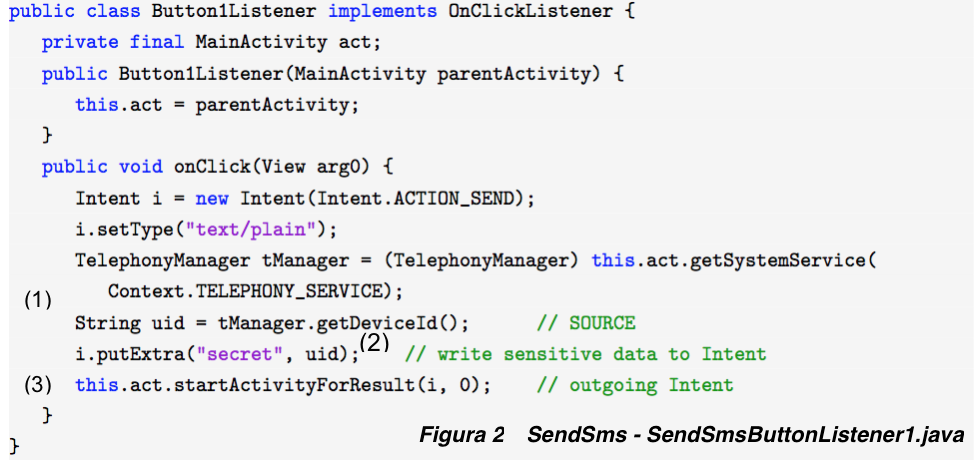
\includegraphics[scale=0.75]{Figura2}
\end{center}

Android \cite{IntAnd} trabaja en Linux, y cada aplicaci�n utiliza un proceso propio. Los dispositivos tienen un �nico foco de ejecuci�n principal, que es la aplicaci�n que est� visible en la pantalla, pero puede tener varias aplicaciones en un segundo plano, cada una con su propia pila de tareas. La pila de tareas es la secuencia de ejecuci�n de procesos en Android. Se componen de actividades que se van apilando seg�n son invocadas, y solo pueden terminarse cuando las tareas que tiene encima est�n terminadas, o cuando el sistema las destruye porque necesita memoria, por lo que tienen que estar preparadas para terminar en cualquier momento. El sistema siempre eliminar� la actividad que lleve m�s tiempo parada. En caso de que el sistema necesitara mucha memoria, si la aplicaci�n no est� en el foco, puede ser eliminada por completo a excepci�n de su actividad principal. \par 
Una de las caracter�sticas principales del dise�o en Android es la reutilizaci�n de componentes entre las aplicaciones, es decir, dos aplicaciones diferentes pueden utilizar una misma componente, aunque est� en otra aplicaci�n para as�, evitar la repetici�n innecesaria de c�digo, y la consiguiente ocupaci�n de espacio. Los componentes son los elementos b�sicos con los que se construyen el proyecto. Hay cuatro tipos, pero las aplicaciones se componen principalmente de actividades. Habr� tantas actividades como ventanas distintas tenga la aplicaci�n. Sin embargo, por si solos, los componentes no pueden hacer funcionar una aplicaci�n. Para ello est�n los "intents". Todos ellos deben declararse en el archivo llamado AndroidManifest.xml (junto con otros elementos que se mostrar�n despu�s) con el mismo nombre que lleve la clase asociada. Por ejemplo, la clase MainActivity, ser� definida en el AndroidManifest con el mismo nombre. 
Los cuatro componentes mencionados antes son:
\begin{description}
\item[Actividades:] Una actividad (o Activity) es la componente principal encargada de mostrar al usuario la interfaz gr�fica. Se define una actividad por cada interfaz del proyecto. Las actividades tienen un ciclo de vida, es decir, pasan por diferentes estados desde que se inician hasta que se destruyen. Sus 3 posibles estados son: Activo: ocurre cuando la actividad est� en ejecuci�n; Pausado: a�n se est� ejecutando y es visible, pero no es la tarea principal; Parado: la actividad est� detenida, no es visible al usuario y el sistema puede liberar memoria.
\item[Servicio:] Los servicios (o service) son tareas no visibles que se ejecutan siempre por debajo, incluso cuando la actividad asociada no se encuentra en primer plano. Tiene un hilo propio (aunque no se pueden ejecutar solo), lo que permite llevar a cabo cualquier tarea, por pesada que sea. No necesita interfaz, a no ser que se pida expl�citamente, en cuyo caso la clase Service la exportar�a. 
\item[Receptores de Mensajes de Distribuci�n:] Tambi�n llamados broadcast receiver, son los encargados de reaccionar ante los eventos ocurridos en el dispositivo, ya sean generados por el sistema o por una aplicaci�n externa.
No tienen interfaz, pero pueden lanzar una activity por medio de un evento. 
\item[Proveedores de contenidos:] Estos proveedores en ingl�s llamados content provider, se encargan de que la aplicaci�n pueda acceder a la informaci�n que necesita, siempre que se haya declarado el correspondiente provider
en el AndroidManifest , compartiendo informaci�n sin revelar estructura u orden interno.
\item[Intents:] Los intents son el medio de activaci�n de los componentes (excepto los content provider). Contiene los datos que describen la operaci�n que desarrollar� el componente a quien va dirigido. 
Pueden ser expl�citos o impl�citos. Los impl�citos no especifican el componente al que va destinado, mientras que el expl�cito, si. 
\item[Intent-filters:] Utilizados �nicamente por los intents impl�citos, los intent-filters definen (y delimitan) qu� tipos de intent puede lanzar la actividad, o qu� tipos de intent puede recibir un broadcast. Por ejemplo, para un intent que no especifica a que actividad va dirigido, se consulta el intent filter de una de ellas, y si lo satisface, el intent lanzar� esa actividad. Se definen en el AndroidManifest con la etiqueta $<$ intent-filter $>$ . La informaci�n que pasan los intents debe estar contenida en la definici�n del intent filter para que la componente pueda ser activada (o pueda recibirlo en el caso del broadcast). Esta informaci�n se compone de tres campos: Action, Data y Category. \par
El campo Action es un string que informa del tipo de acci�n llevada a cabo. Las acciones pueden ser dadas por la clase Intent, por una API de Android o definidas por el dise�ador. \par
el campo Data contiene la informaci�n del identificador (URI) del dato que se asocia a la acci�n y del tipo de ese dato. Es importante la coherencia ya que si la acci�n requiere un dato de tipo texto, un intent con un dato de tipo imagen no podr�a ser lanzado.\par
Por �ltimo, el campo Category es un string (cadena de caracteres) que contiene informaci�n adicional sobre el tipo de componente al que va dirigido el intent. La lista de categor�as esta incluida en la clase Intent.
\item[AndroidManifest:]  este fichero es un documento xml en el que se declaran los elementos de la aplicaci�n, as� como sus restricciones, permisos, procesos, acceso a datos e interacciones con elementos de otras aplicaciones. Cada elemento se declara con una etiqueta �nica. No debe confundirse este documento con el xml asociado a cada actividad. Los elementos gr�ficos y distribuci�n de la pantalla ser�n definidos para cada actividad dentro de su xml, pero no en el AndroidManifest. 
\end{description}

Cada aplicaci�n es comprimida en un paquete APK, lo que permite su distribuci�n e instalaci�n. Estos paquetes contienen una colecci�n de archivos, recursos, permisos, entre otras cosas, como muestra la siguiente figura. \par 

\begin{center}
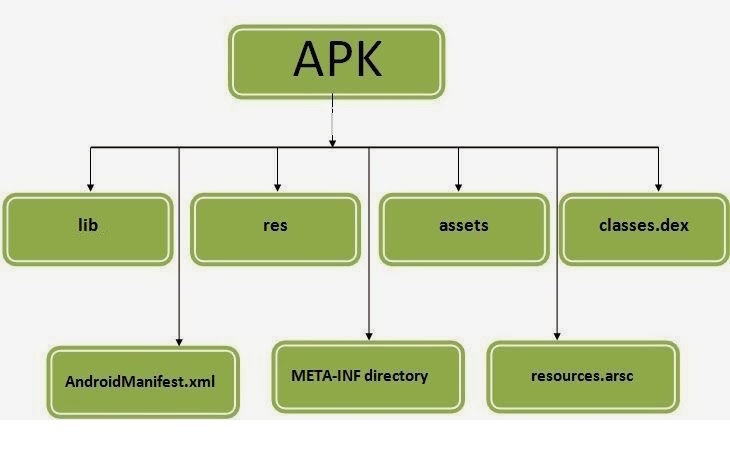
\includegraphics[scale=0.5]{Figura3}
\end{center}

\section{Ejemplo Motivador}

La comunicaci�n entre las aplicaciones es muy com�n y necesario para cumplir con sus objetivos. Esta comunicaci�n la llevan a cabo principalmente mediante el uso de intents. Un ejemplo de ello es una foto, la cual puede fluir a trav�s de diferentes aplicaciones: es sacada por la c�mara y almacenada, luego es editada por alguna aplicaci�n de edici�n para posteriormente ser compartida a trav�s de alguna red social.\par

\begin{center}
 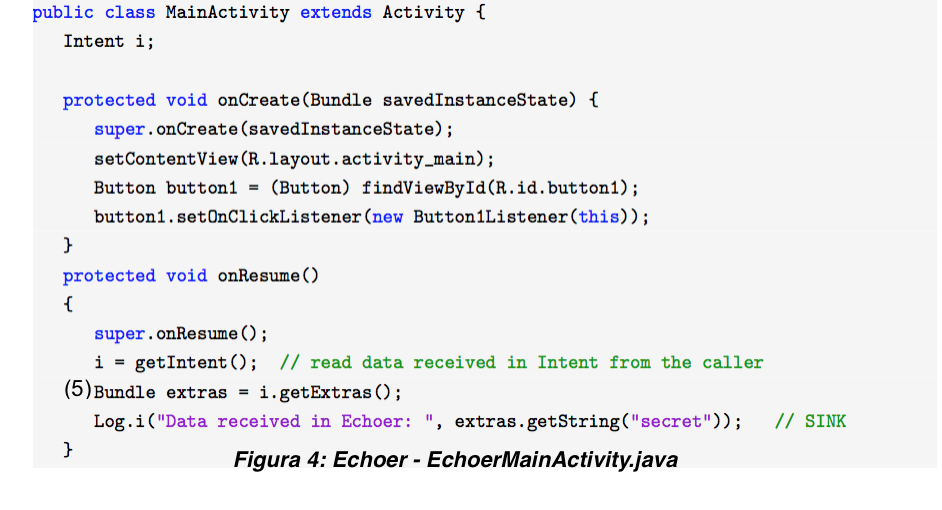
\includegraphics[scale=0.75]{Figura4}
 \end{center}
En la siguiente imagen se muestra un ejemplo donde informaci�n sensible puede fluir desde un source a un sink, y en su "viaje", pasar por m�ltiples aplicaciones que pueden ver y modificar su informaci�n: \par

\begin{center}
 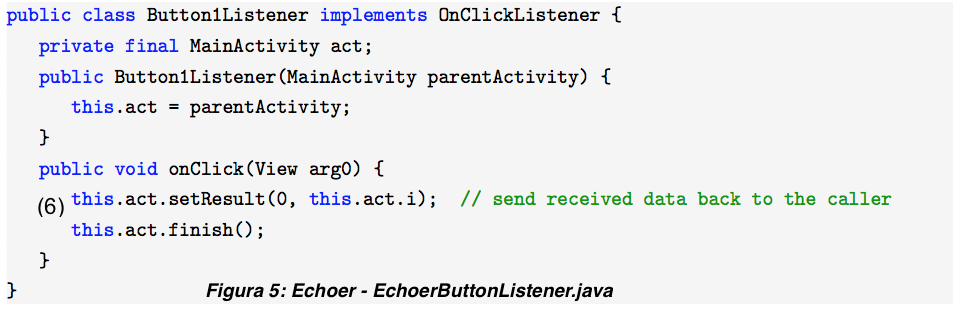
\includegraphics[scale=0.75]{Figura5}
 \end{center}
 
Aqu� la aplicaci�n SendSms obtiene Device Id (Figura 6: (1)), lo guarda en un intent (Figura 6: (2)) y luego lo env�a mediante el m�todo startActivityForResult (Figura 6: (3)) para iniciar una nueva actividad. Dicho intent es impl�cito, es decir, no tiene un destinatario preestablecido, por lo que el sistema operativo se encarga de comprobar que aplicaciones pueden manejarlo (mediante la comprobaci�n de sus archivos manifest). En este ejemplo, la aplicaci�n elegida fue Echoer.apk debido que su Manifest cumpl�a con los requisitos (Figura 10: (4)). �sta aplicaci�n recibe el intent, lo guarda en un campo de la clase MainActivity (Figura 8: (5)), y luego de que se oprima el bot�n "button1", la informaci�n que tenia el intent es enviada de vuelta a la aplicaci�n SendSms (Figura 9: (6)), para que este �ltimo envi� el mensaje (Figura 7: (7)). \par
En el escenario descripto, el source (deviceId), es informaci�n privada del dispositivo, puede llegar a dos sinks diferentes: uno de ellos es el Sms saliente y el otro sink es el Log, y de acuerdo a los niveles que se le asignen a estos �ltimos, los flujos puede o no producir una violaci�n de seguridad. \par
Las figura Figura 8 (5) y Figura 9 (6) muestran como fluye la informaci�n al Log escribiendo el contenido del intent recibido.

\par
\begin{center}
 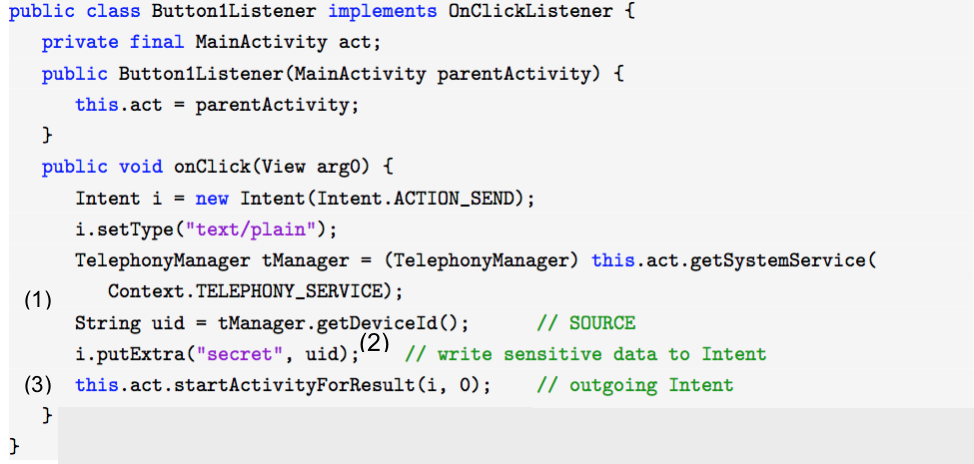
\includegraphics[scale=0.8]{Figura6}
 \end{center}
\par
\begin{center}
 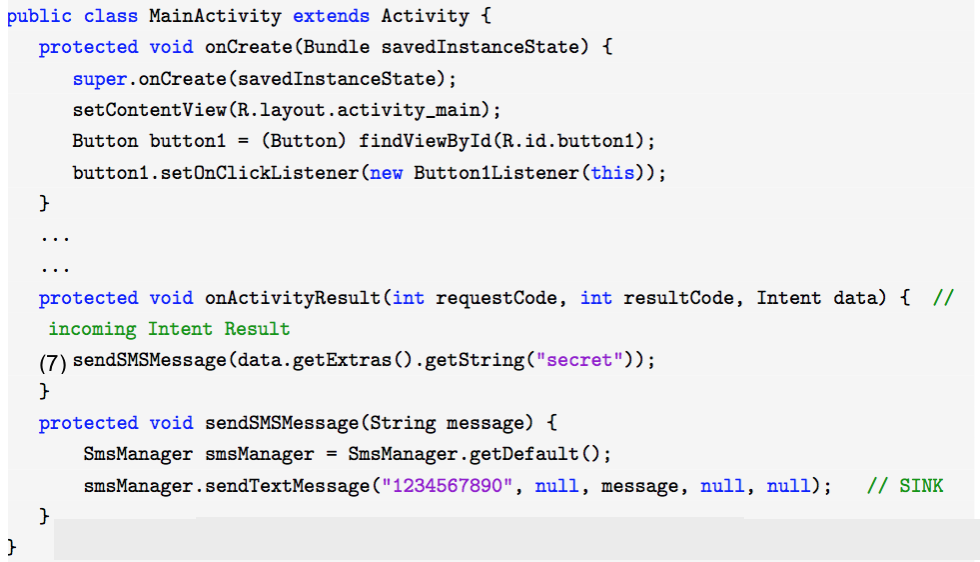
\includegraphics[scale=0.8]{Figura7}
 \end{center}
\par
\begin{center}
 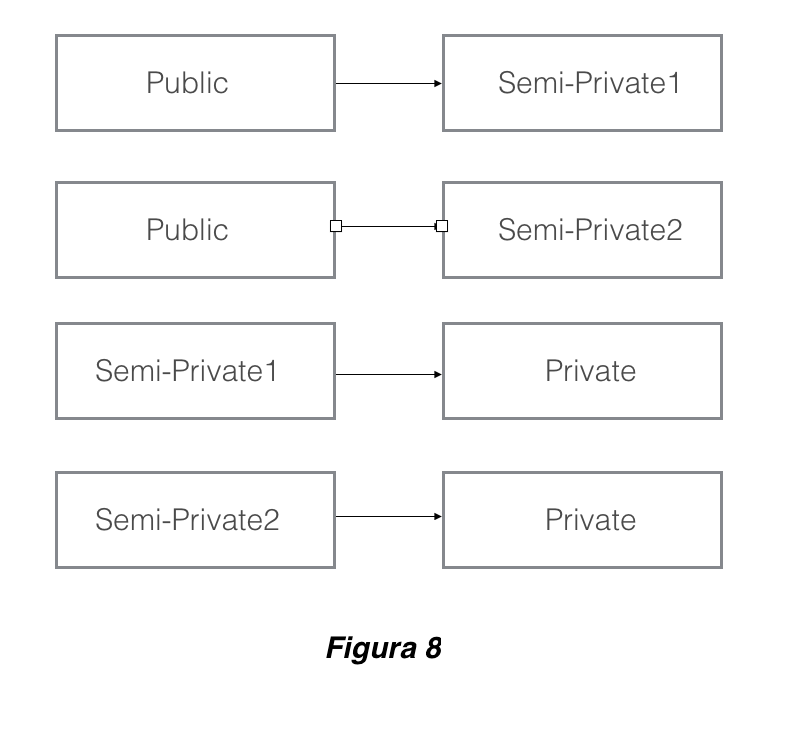
\includegraphics[scale=0.8]{Figura8}
 \end{center}
\par
\begin{center}
 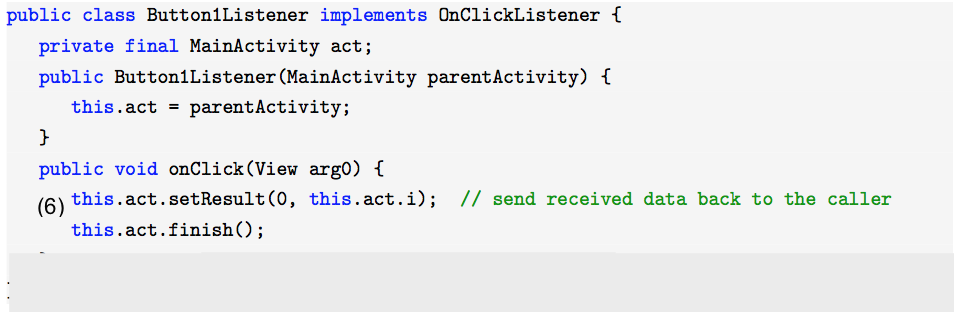
\includegraphics[scale=0.8]{Figura9}
 \end{center}
\par
\begin{center}
 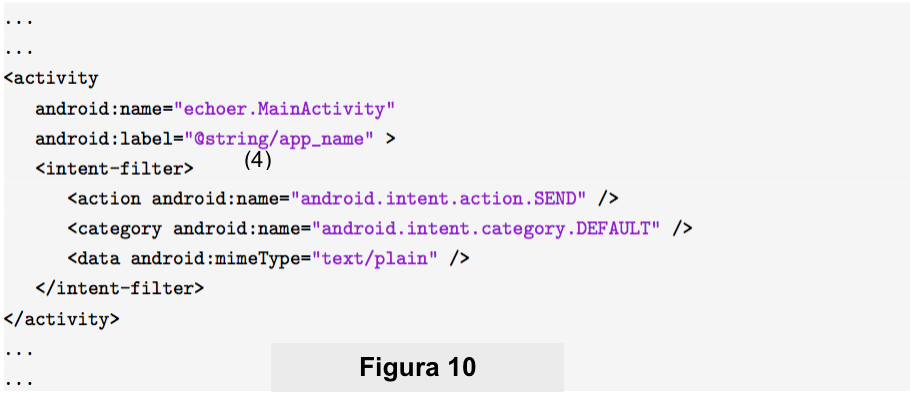
\includegraphics[scale=0.8]{Figura10}
 \end{center}
 
En este ejemplo se representa lo que sucede en muchas aplicaciones ya sea por mala intenci�n o por descuidos: la aplicaci�n SendSms quiere comunicarse con otro componente de s� misma, enviarle informaci�n para que �ste lo trate seg�n corresponda, para lo cual manda un intent con dicha informaci�n. A continuaci�n, Echoer recibe el intent, filtra la informaci�n, y luego env�a otro intent para que la aplicaci�n inicial siga con su normal funcionamiento. Aqu� SendSms no sabe que su informaci�n fue vista y tratada por otra aplicaci�n. Este flujo es detectado por Didfail.\par

\section{Herramientas de an�lisis est�tico}

La herramienta detallada en este informe se construy� sobre Didfail, la cual a su vez utiliza Flowdroid y Epicc. \par

\subsection{Flowdroid}

Flowdroid \cite{Flowdroid} es una herramienta de an�lisis est�tico para aplicaciones Android, de c�digo abierto. La cual reduce el programa a un simple gr�fico que modela el ciclo de vida de las aplicaciones de Android. \par
Analizar dichas aplicaciones es mas complicado que analizar un programa en java  porque estos corren sin el framework de Android, tienen un simple punto de entrada (el m�todo main). En cambio, las aplicaciones Android, pueden tener multiples puntos de entradas, llamados impl�citamente por el framework. Flowdroid resuelve este problema creando un m�todo llamado dummymain(), el cual emula el ciclo de vida de las aplicaciones incluyendo todas las llamadas impl�citas que pueden ocurrir.\par
Flowdorid puede detectar precisamente solo flujos de datos intraprocedurales, ya que los interprocedurales incluyen intents, service, entre otros.\par

\subsection{Epicc}

Epicc analiza la comunicaci�n entre componentes de manera precisa y efectiva, por lo que se podr�a decir que es un complemento a lo realizado por Flowdroid. \par
Epicc identifica propiedades (tales como action, category and data MIME type) de los intents que pueden ser enviados y recibidos por los diferentes componentes.

\subsection{Didfail}

DidFail (Droid Intent Data Flow Analysis for Information Leakage) \cite{Didfail} usa el an�lisis est�tico para detectar potenciales fugas de information sensible entre un conjunto de aplicaciones Android. DidFail combina FlowDroid y Epicc para realizar un seguimiento de los flujos de datos tanto entre componentes como dentro de cada componente de un conjunto de aplicaciones. DidFail tiene dos fases en el an�lisis:
\begin{itemize}
\item Dado un conjunto de aplicaciones, primero determina el flujo de datos individualmente por cada una, y las condiciones en las que estos son posibles.
\item Luego, bas�ndose en los resultados de la primer fase, enumera los flujos de datos potencialmente peligrosos habilitados por las aplicaciones en su conjunto.
\end{itemize}

En los cap�tulos siguientes se presenta como a partir de la salida que proporciona Didfail, y mediante modificaciones en dicha herramienta, se le dan niveles a los m�todos involucrados en los flujos, se chequean si se produce violaciones de seguridad de acuerdo al orden establecido entre los niveles, ignorando aquellos m�todos que son considerados excepciones, y las opciones para introducir dicha informaci�n.\par
 
% 
 \lhead{\emph{Dise�o}}
\graphicspath{{Imagenes/}} 

\chapter{Dise�o}

El objetivo es que a partir de la informaci�n que nos proporciona la herramienta Didfail (con algunas modificaciones) y la informaci�n ingresada por el usuario como los niveles de seguridad con los que se va a trabajar, el orden parcial que los relaciona, las excepciones, y la asignaci�n de niveles tanto a los source como a los sinks, identificar cual es el flujo de informaci�n que viola lo anterior mencionado en caso de que exista o informar la ausencia de dichas violaciones y brindar una posible asignaci�n de niveles a los source y sinks que no fueron proporcionados por el usuario.
Dicho an�lisis puede considerarse dividido en dos etapas: la primera consiste en la recopilaci�n de informaci�n necesaria para efectuar el an�lisis y la segunda, a partir de la anterior, generar la informaci�n saliente, calcularla e informarla a trav�s de la salida preestablecida. 

\section{Escenario de ejemplo}

\subsection{Informaci�n obtenida a trav�s de Didfail}

Un ejemplo de los escenarios a analizar por la herramienta es el que muestra la imagen que sigue (Figura 7), donde el componente 1 env�a datos al componente 2, este ultimo los recibe y env�a otros como respuesta. Por otro lado, el componente 3 interact�a con el componente 2 de manera similar. Vale aclarar que estos componentes pueden o no ser parte de una misma aplicaci�n, lo cual no cambia el resultado en el an�lisis.

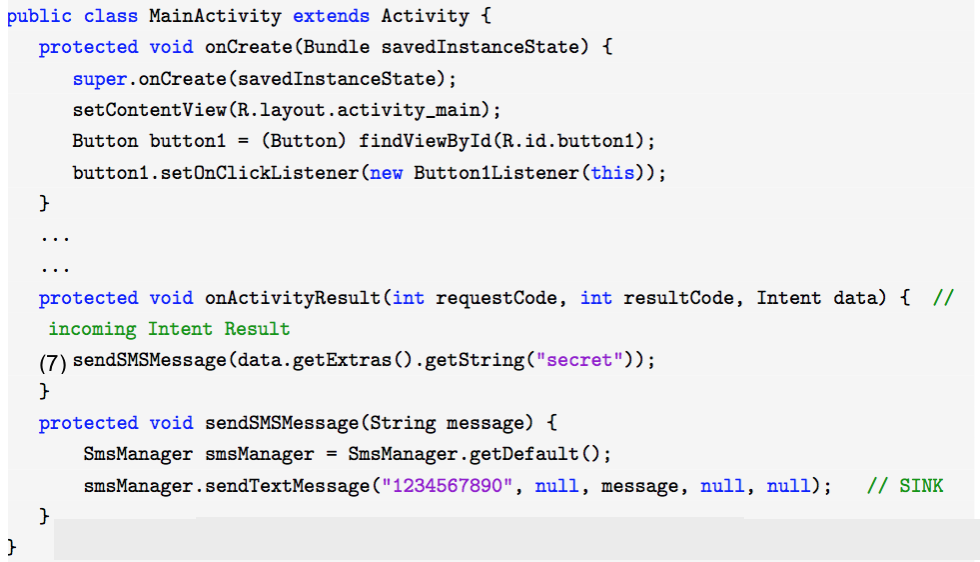
\includegraphics[scale=0.75]{Figura7}
\par

En el escenario de la figura 7, Didfail determina que la informaci�n puede fluir  de  C1 a C2, de C2 a C1, de C3 a C2 y de C2 a C3 de manera directa, pero tambi�n pueden suceder flujos de C1 a C3 y de C3 a C1, en el caso de que C2 al recibir la informaci�n de, por ejemplo, C1, la guarde en alg�n campo y posteriormente la envi� como respuesta a C3, luego de recibir un intent proveniente de este ultimo.\par
Estos flujos son originalmente representados de a pares, donde el componente izquierdo representa el source del flujo (quien env�a el intent) y el componente derecho representa el sink del flujo (quien recibe el intent). Por ende, el resultado seria (source1, sink3), (source3, sink1), (source1, sink1) y (source3, sink3). \par
A partir de las modificaciones que afectaron a Didfail, los source y sink tienen un campo llamado level, que permite, una vez calculado el flujo, comparar los niveles y ver si se corresponden con el orden entre ellos (vease 3.1.2)

\subsection{Informaci�n obtenida a trav�s de archivo de configuraci�n �nicamente}

Otra informaci�n necesaria para efectuar el an�lisis son los niveles de seguridad y el orden que los relaciona, el cual debe ser un orden parcial como requisito excluyente, vease Figura 8. \par
Aqu� no es necesario dar las relaciones transitivas (por ejemplo Public - Private) ni tampoco las relaciones reflexivas (Public - Public), las cuales deben estar presentes para cumplir con el requisito de orden parcial pero, para hacer el trabajo del usuario mas simple,  las relaciones reflexivas y transitivas son calculadas autom�ticamente.\par
Los motivos por el que la relaci�n entre los niveles debe ser de orden parcial son:
\begin{description}
\item[Reflexividad:] La reflexividad, como indica su definici�n, cualquier elemento del orden se precede a si mismo. Esto es necesario ya que al momento de comprobar el cumplimiento o no de un flujo de informaci�n, si tanto el source como el sink tienen el mismo nivel de seguridad, no hay violaci�n. Si la relaci�n no fuese reflexiva, y por ejemplo, la relaci�n``Public - Public'' no esta presente, la existencia de un flujo entre m�todos que tienen el nivel ``Public'' asignado ser� considerado una violaci�n de seguridad. 
\item[Transitividad:] Esta propiedad es requerida ya que, al permitirse muchos niveles distintos, se puede dar que exista, por ejemplo, la relaci�n ``Public - SemiPrivate'' y ``SemiPrivate - Private'' donde, si la relaci�n ``Public - Private'' no forma parte del orden, un flujo que vaya desde el nivel ``Public'' al nivel ``Private'' ser�a considerado una violaci�n de seguridad. Esto es un problema ya que sabemos que ``Public'' precede en el orden a ``SemiPrivate'' y este ultimo precede a ``Private'', por lo que el flujo ``Public - Private'' no debe ser una violaci�n. Esto se soluciona garantizando que el orden entre los niveles sea transitivo.
\item[Antisimetr�a:] Esta propiedad evita ciclos en el orden, lo cual es claramente necesario debido a que en caso de no cumplirse, todos los niveles que participan en un ciclo (por la transitividad) podr�an ser reemplazado por uno solo sin modificar los resultados de los an�lisis que los usen.
\end{description}
\par

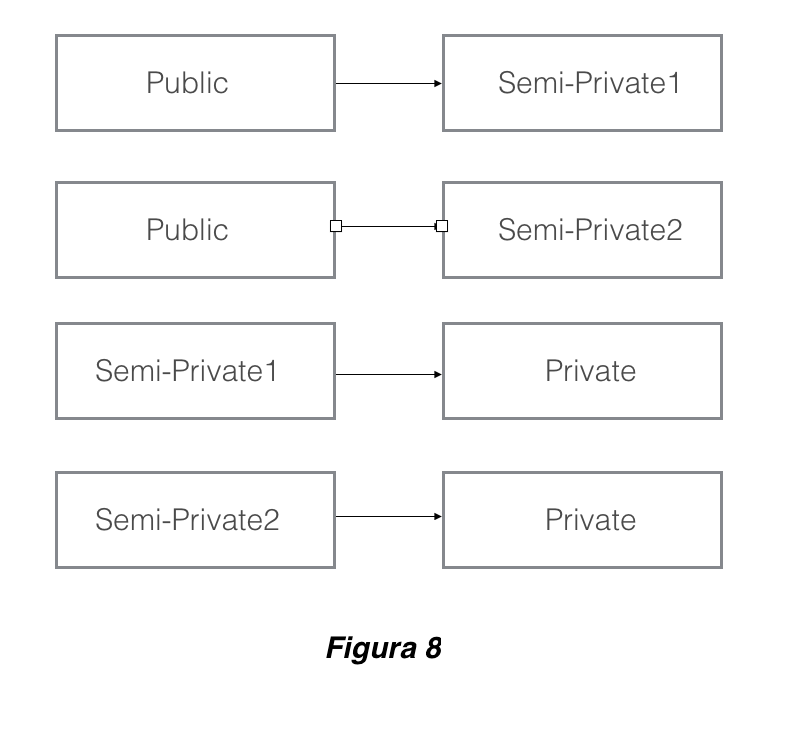
\includegraphics[scale=1]{Figura8}

\subsection{Informaci�n obtenida mediante gui o archivos de configuraci�n}

Las entradas que deben proporcionarse a la herramienta que caben en esta clasificaci�n corresponden a la asignaci�n de niveles a m�todos y las excepciones.
La asignaci�n de niveles a m�todos podr�an ser como se muestra en la figura 9, por ejemplo. 

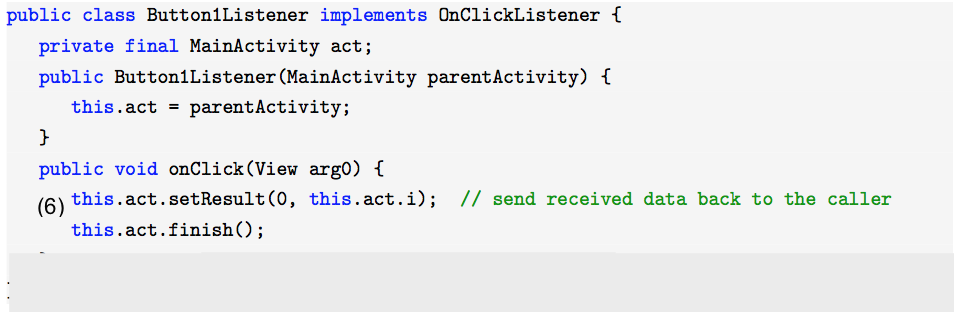
\includegraphics[scale=0.75]{Figura9}
\par

Aqu�, al m�todo source1 se le asigna el nivel privado, lo cual se interpreta de la siguiente manera: la informaci�n que obtiene la ejecuci�n del m�todo source1 es informaci�n privada que, de acuerdo al orden de los niveles anteriores, no debe llegar a ser argumento de alguno de los m�todos con un nivel menor, como son Public, Semi-private1 o Semi-private2. \par
En cuanto a la interpretaci�n de la asignaci�n a sink1 corresponde a que la informaci�n que tiene el m�todo sink1 como argumento, luego de la ejecuci�n de �ste, llega a lugares considerados "Private".\par
Un ejemplo concreto puede ser, que dado el m�todo getLatitud(), el cual obtiene la ubicaci�n del dispositivo considerada normalmente como informaci�n privada, se le asigna el nivel  ``Private''. Por otro lado, la informaci�n que es enviada via sms (mediante el m�todo sendSms()) normalmente es considerada p�blica ya que puede llegar a distintas personas. Teniendo en cuenta este escenario, si existe el flujo (getLatitud, sendSms), existe una violaci�n de seguridad donde informaci�n privada arriba a lugares p�blicos.\par
En el caso de las excepciones, pueden ser:\par
\begin{description}
\item[source1 a sink3]
\end{description}
Esto significa que si Didfail detecta un flujo de source1 a sink3, sin  importar los niveles que estos tengan asignado, el flujo es ignorado, y no provoca violaciones de seguridad.\par
Un ejemplo concreto del uso de excepciones que se puede mencionar es el caso en el que una aplicaci�n dada requiere que el usuario se identifique antes de proveerle sus funcionalidades. Para ello el usuario introduce su contrase�a, la cual es considerada informaci�n privada. En el caso de que la contrase�a introducida sea err�nea, la aplicaci�n responder� indicando el fallo y posiblemente pidiendo el reingreso de �sta. Aqu� surge un inconveniente, donde un componente que recibe informaci�n privada, la trata y responde a, posiblemente, un componente considerado p�blico, como por ejemplo, la ventana informando que la contrase�a es incorrecta. Si bien la ventana podr�a contener la contrase�a ingresada, lo cual seria claramente una fuga de informaci�n, tambi�n puede responder simplemente el mensaje de error o �xito. Para situaciones como estas, la herramienta le deja la decisi�n al usuario, dandole la posibilidad de ignorar la violaci�n de seguridad mediante el uso de excepciones.\par
Otro escenario posible puede darse en el caso de que un m�todo que participe en alguna excepci�n no tenga nivel asignado por el usuario y deba ser calculado por la herramienta. Aqu�, si durante el an�lisis se encuentra el flujo indicado por la excepci�n, �ste no va a limitar la asignaci�n de un nivel al m�todo, es decir, si por ejemplo, el flujo va de ``privado'' a ``variable1'' (donde ``privado'' es el nivel supremo del orden de los niveles y ``variable1'' es el m�todo que no tiene nivel asignado), al momento de calcular el nivel del m�todo ``variable1'' no se tendr� en cuenta dicho flujo, es decir, no debe ser mayor o igual a ``privado''. \par

\section{Etapa 1}

En esta etapa, se recolecta toda la informaci�n necesaria para efectuar el an�lisis. �sta puede ser provista por dos v�as: Mediante la interfaz de usuario o mediante archivos de configuraci�n, dependiendo del script que sea utilizado para ejecutar la herramienta. \par
Dado el escenario anterior, se reemplaza cada m�todo en los flujos por su nivel de acuerdo a la asignaci�n brindada por el usuario, y en caso de que el m�todo no tenga una asignaci�n, ser� considerado variable y su nivel depender� luego de los dem�s para evitar la violaci�n del orden de los niveles. Esto es, puede darse el caso de que exista un nivel, el cual se le asigne al m�todo variable y luego el chequeo no de error. O por el contrario, puede ocurrir que no exista dicho nivel y por lo tanto el sistema informar� la violaci�n.\par
En el caso de los niveles de seguridad, se le agregan todos las relaciones necesarias para que el orden resultante sea un orden parcial. De igual manera, dicha relaci�n puede resultar no ser del orden requerido por el no cumplimiento de la antisimetr�a (requisito para ser orden parcial).\par
Por otro lado, tambi�n se requiere que los m�todos participantes en las excepciones deben existir (pertenecer a la API de la versi�n de Android que la herramienta utiliza). \par
En el caso de las asignaciones de niveles a m�todos, los m�todos deben cumplir el mismo requisito que los de las excepciones y adem�s, el nivel que se le asigna a cada uno debe pertenecer al orden generado con anterioridad.
En cualquier caso que no se cumplan los requisitos antes mencionados, se generar� un error y se abortara la ejecuci�n.\par

\section{Etapa 2}

Una vez que se cuenta con toda la informaci�n necesaria, se lleva a cabo el chequeo de los flujos de informaci�n. La idea general de dicho chequeo  es comprobar que la informaci�n no fluya a lugares ``m�s p�blicos'' que de donde sali�, es decir, que los niveles de los m�todos con los que esta informaci�n es recopilada no sean menores (precedan en el orden de los niveles) a los niveles de los m�todos donde puede llegar dicha informaci�n. Pero, dado que no todos los m�todos pueden tener nivel asignado, es necesario la previa asignaci�n de un nivel, para luego proceder con el chequeo. \par
Si se tomara como entrada a la etapa 2 el escenario de la figura 7, 8 y 9, por ejemplo, ``source1'' tiene asignado el nivel ``Private'', adem�s, como sabemos que la informaci�n obtenida por ``source1'' puede llegar a ``sink3'', y este �ltimo tiene nivel ``Semi-private3'' y dado que el orden de los niveles indica que ``Semi-private3'' es menor que ``Private'', se estar�a produciendo una violaci�n de seguridad. Pero, como dicho flujo esta presente en las excepciones, �ste es descartado.\par
Otro caso que puede ocurrir es que la informaci�n vaya de un nivel menor a uno mayor o el caso que los niveles de seguridad sean iguales, en ambos casos no hay problemas de seguridad. Teniendo en cuenta el ejemplo, este caso es representado por el flujo ``source1 - sink1''.\par
Una ultima alternativa seria, por ejemplo, el caso de que el flujo se d� entre ``Semi-private1'' y ``Semi-private2'': Aqu�, los niveles son incomparable en el orden, lo que tambi�n deriva en una violaci�n de seguridad (``source3 - sink3'').\par


 
% 
 \lhead{\emph{Resultados Experimentales}}
\graphicspath{{Imagenes/}} 
\chapter{Resultados Experimentales}

En este capitulo se muestra un ejemplo del an�lisis mediante el uso de tres aplicaciones diferenciando las dos formas que tiene el usuario de brindar datos a la herramienta.\par

\section{Descripci�n de aplicaciones a analizar}

\begin{description}
\item[SendSMS.apk:] Esta aplicaci�n filtra el \textit{device ID} del usuario a trav�s de un mensaje de texto. Lee el \textit{Device ID} y a continuaci�n lo a�ade a un intent utilizando el m�todo \textit{putExtra()}, acto seguido env�a el intent a trav�s del m�todo \textit{startActivityForResult()} permitiendo a otra aplicaci�n recibirlo y responder. Una vez recibida la respuesta, la aplicaci�n filtra los datos a un mensaje.
\item[Echoer.apk:] Esta aplicaci�n recibe un intent usando el m�todo \textit{getIntent()}, escribe los datos recibidos en el \textit{Log} y por ultimo, env�a los datos de vuelta usando \textit{setResult()}.
\item[WriteFile.apk:] Esta aplicaci�n es similar a \textit{SendSMS}, excepto que lee la ubicaci�n del dispositivo y la fuga a un archivo.
\end{description}
\par

\section{Datos}

\subsection{Jerarqu�a de niveles de seguridad}

En este ejemplo se usaron los niveles de seguridad que muestra la Figura 19. En ella se puede observar a modo de comentario la representaci�n gr�fica del orden generado.\par

\begin{center}
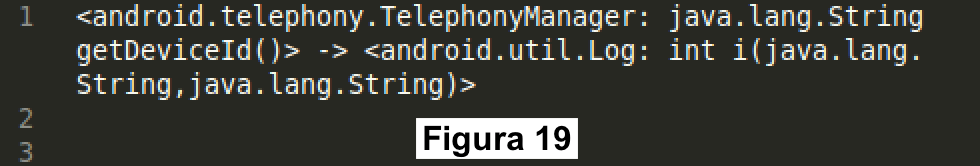
\includegraphics[scale=0.5]{Figura19}\par
Figura 19: Ejemplo de definici�n de orden parcial entre niveles de seguridad.
\end{center}

\subsection{Asignaci�n de niveles}

Para mostrar el funcionamiento de la herramienta solo se le asigna niveles a dos categor�as como muestra la Figura 20, ya que, como se ah mencionado con anterioridad, no es necesario darle niveles a todas las categor�as participantes en los flujos de informaci�n, los restantes niveles de seguridad ser�n inferidos por el an�lisis. \par

\begin{center}
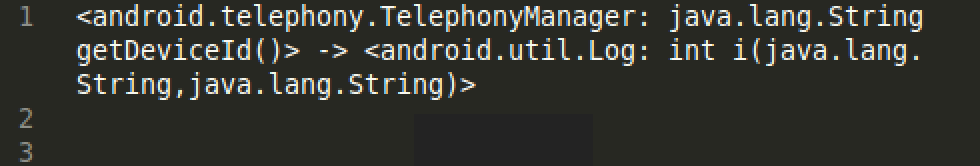
\includegraphics[scale=0.75]{Figura20}\par
Figura 20: Ejemplo de asignaci�n de niveles a categor�as de sources y sinks.
\end{center}

\subsection{Excepciones}

La excepci�n de la Figura 21 hace que se ignore el flujo del \textit{device ID} del usuario al \textit{Log}.\par

\begin{center}
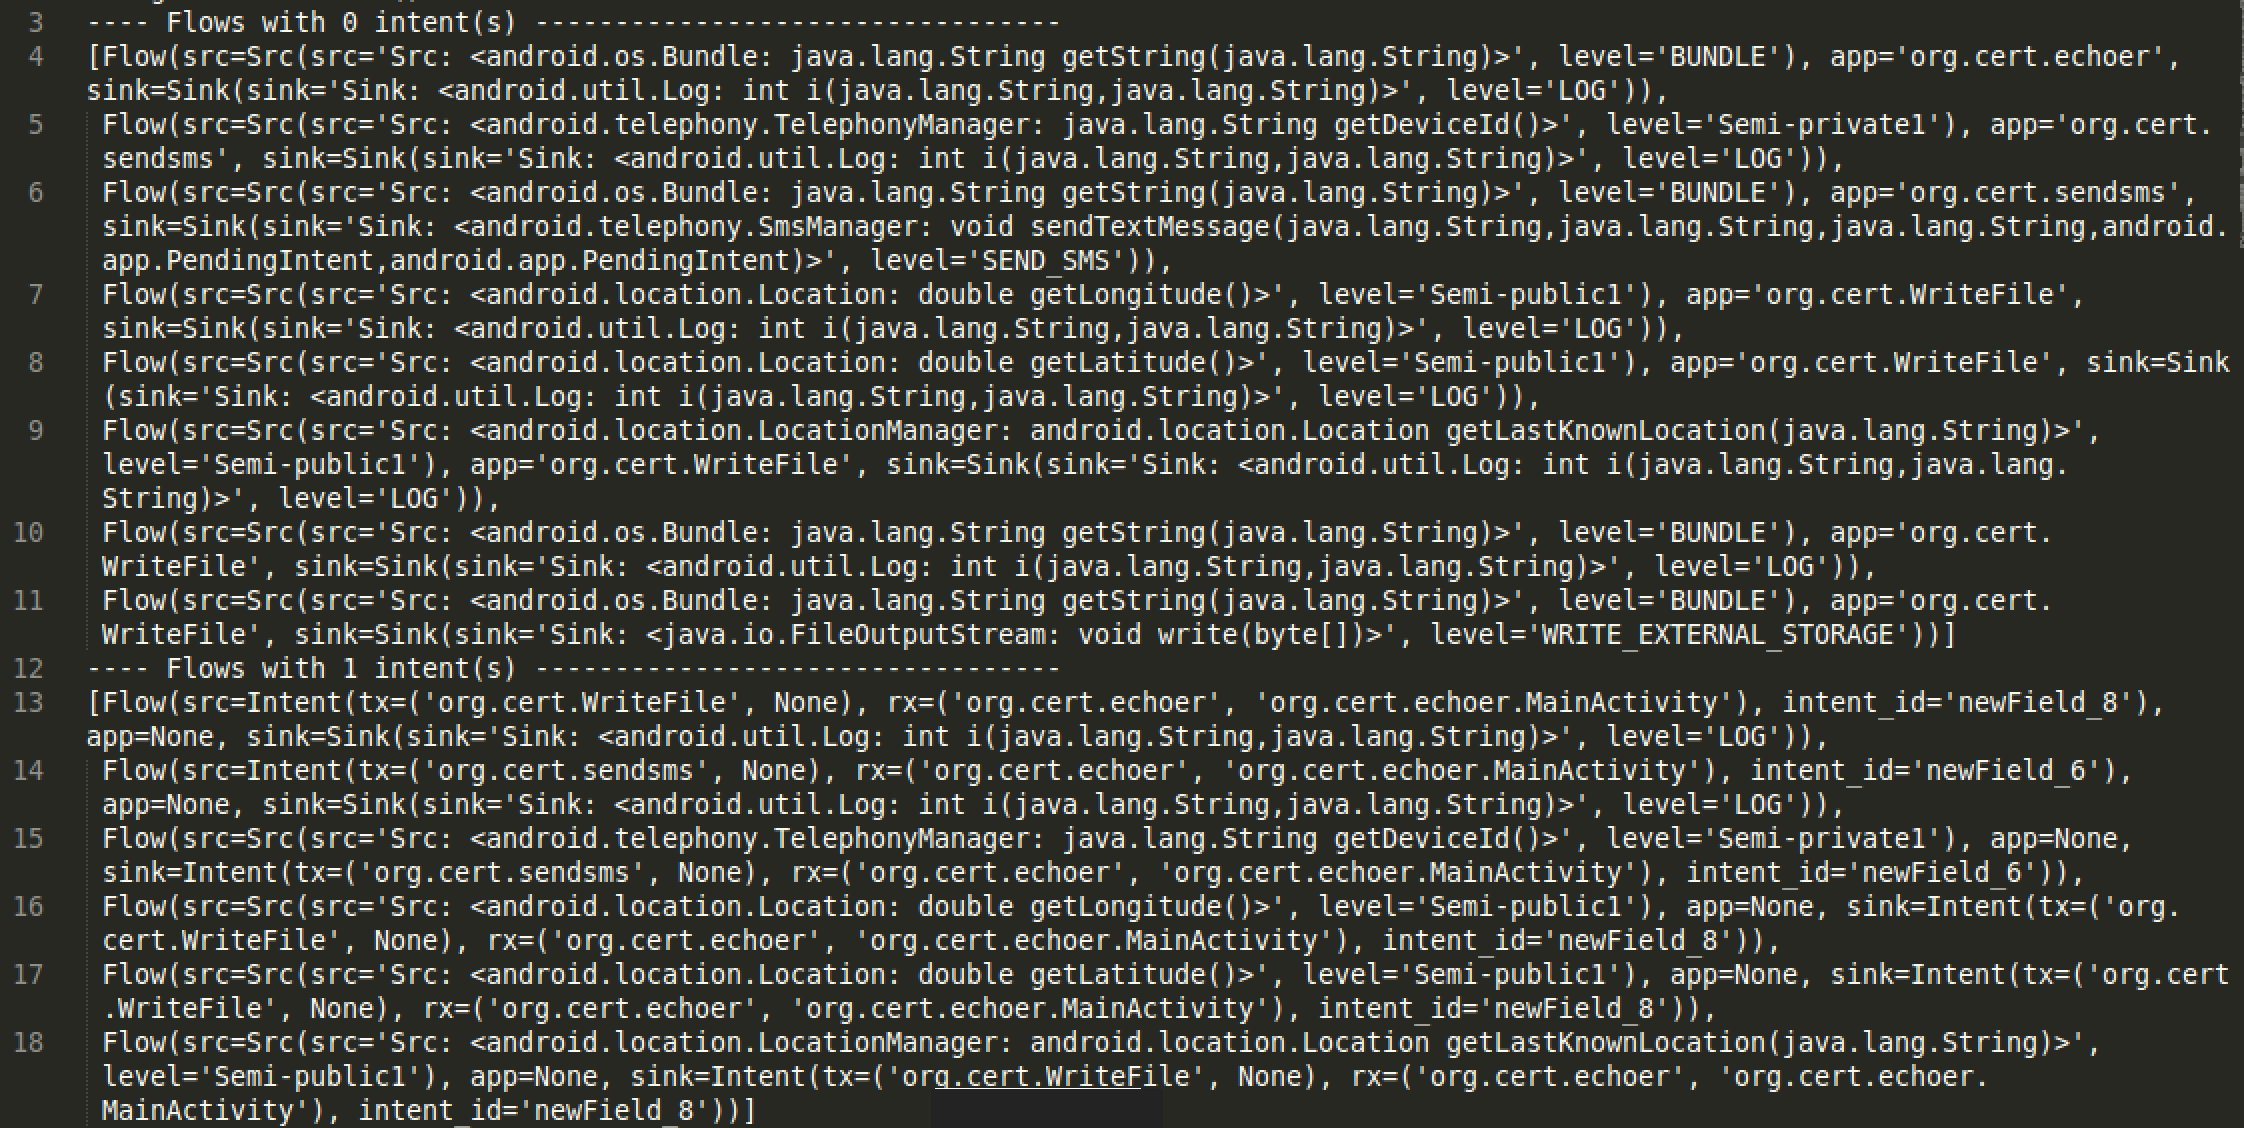
\includegraphics[scale=0.75]{Figura21}\par
Figura 21: Ejemplo de definici�n de excepci�n.
\end{center}

\subsection{Didfail modificado}

Las figuras 22 muestran los flujos de informaci�n, los m�todos que participan y los niveles de seguridad tiene cada uno asignado. El formato mostrado se corresponde con una lista de diccionarios (estructura de datos proporcionada por el lenguaje python), donde cada uno contiene el soruce y el sink del flujo, y en estos �ltimos se especifica el m�todo y el nivel de seguridad correspondiente. En el caso de la figura 22a se puede observar que, por ejemplo, el an�lisis detect� un flujo que va del m�todo \textit{android.telephony.TelephonyManager: java.lang.String getDeviceId()} con nivel \textit{semi-private1} al sink \textit{android.util.log: int i(java.lang.String, java.lang.String)} con nivel variable \textit{LOG} y por lo tanto �ste nivel variable no podr� ser m�s p�blico que el nivel del source antes mencionado. \par
En el caso de la figura 22b el source o el sink corresponde a un intent, el cual es identificado por un id y en el caso de la figura 22c, ambos componentes del flujo son intents.\par

\begin{center}
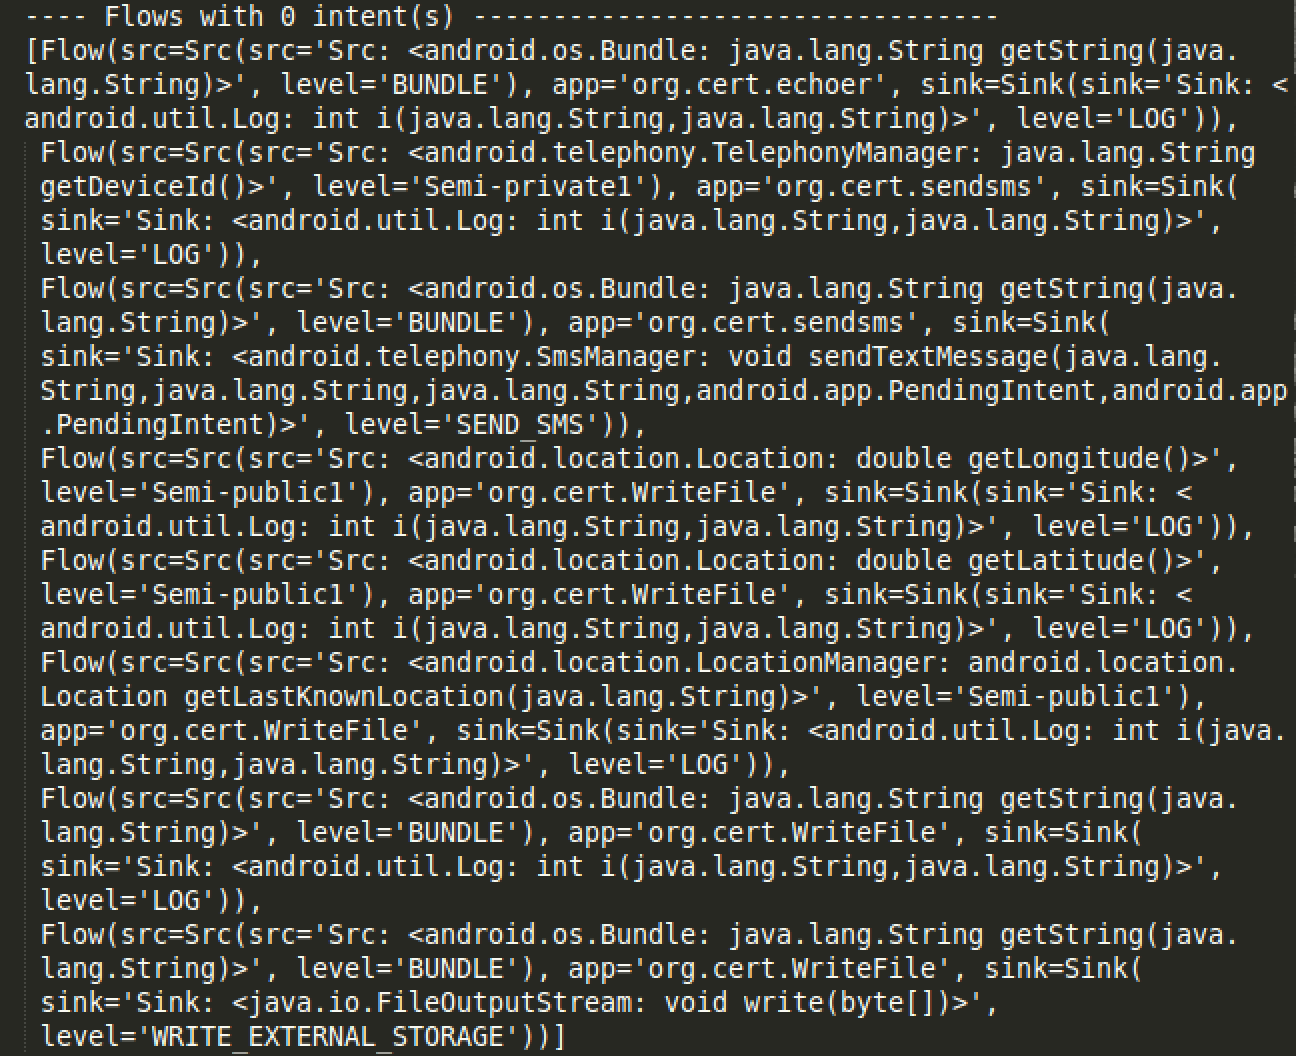
\includegraphics[scale=0.60]{Figura22a}\par
Figura 22a: Flujos que no involucran intents.
\end{center}

\begin{center}
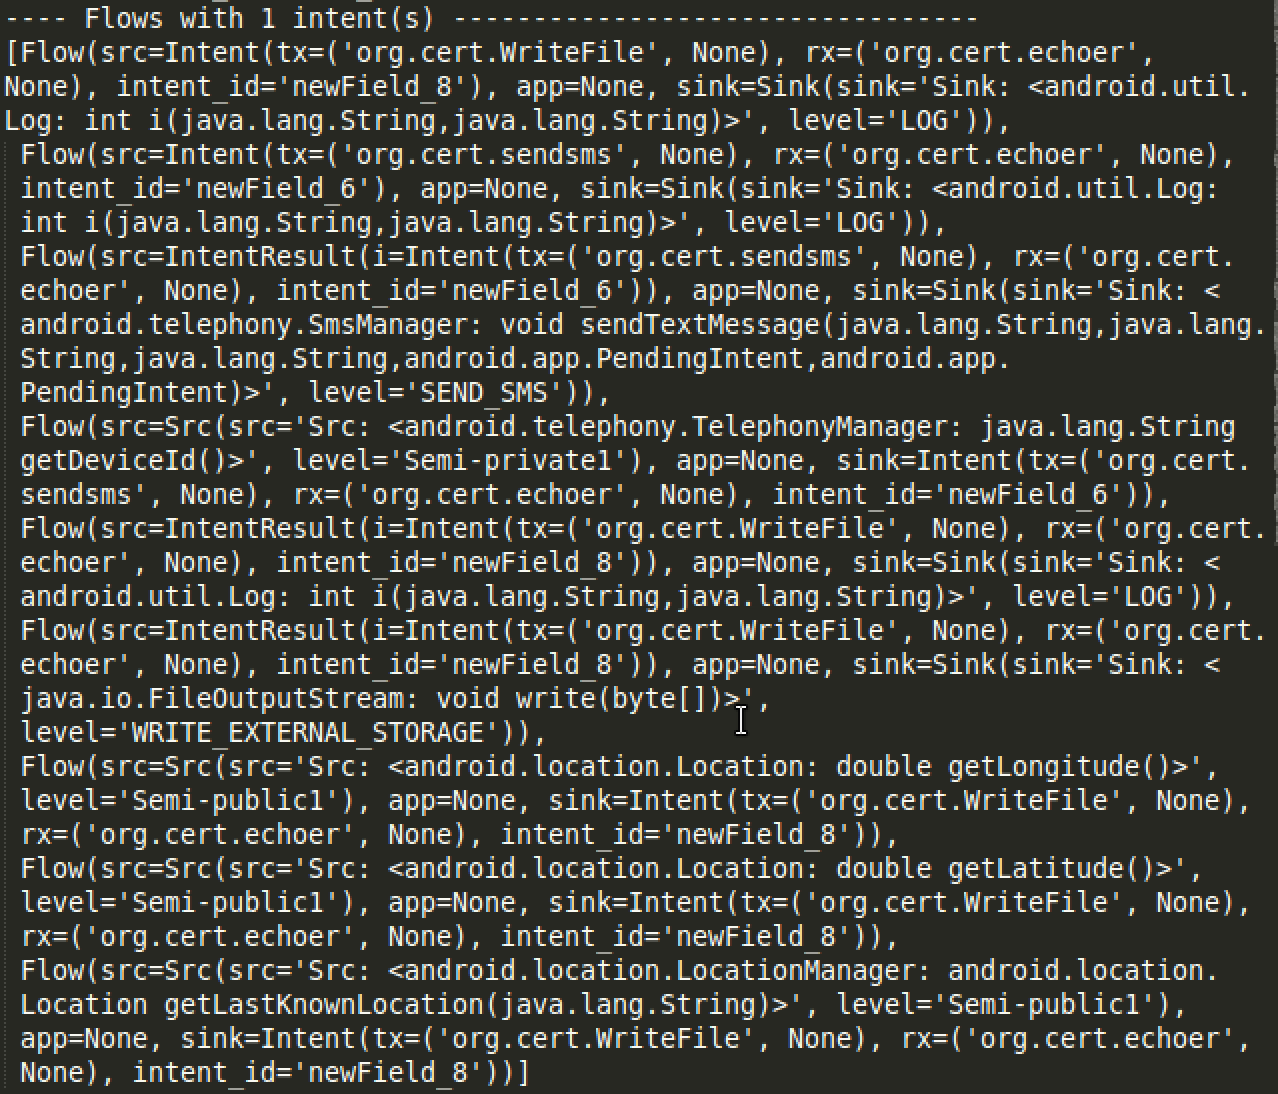
\includegraphics[scale=0.60]{Figura22b}\par
Figura 22b: Flujos con un intents involucrado.
\end{center}

\begin{center}
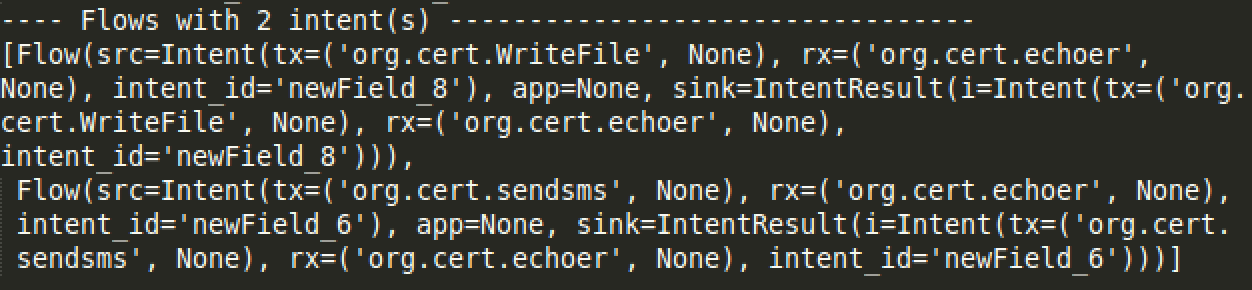
\includegraphics[scale=0.60]{Figura22c}\par
Figura 22c: Flujos con dos intents involucrados.
\end{center}

\section{Resultados obtenidos}

Los resultados obtenidos (Figura 23) muestran que no se producen flujos de informaci�n que viole los niveles de seguridad. Adem�s muestra el menor nivel posible, con respecto a los niveles de seguridad, a cada categor�a que no ten�an nivel asignado.\par
La salida tambi�n incluye los Intent lanzados por las aplicaciones. En el conjunto actual de aplicaciones, estos ya fueron utilizados para el an�lisis y no agrega informaci�n en la salida, pero teniendo en cuenta una posible adici�n de otra aplicaci�n al conjunto, el usuario tiene la posibilidad de ver el nivel de la informaci�n que la nueva aplicaci�n puede obtener (en caso de que su archivo manifest as� lo permita).\par

\begin{center}
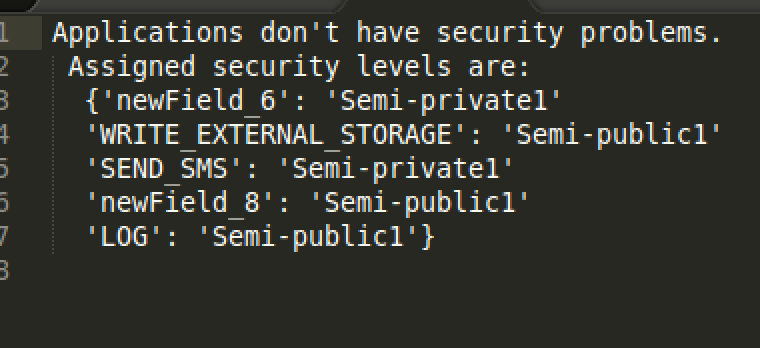
\includegraphics[scale=0.9]{Figura23}\par
Figura 23: Resultados del an�lisis.
\end{center}

El nivel asignado a la categor�a \textit{Log} merece una aclaraci�n. Como se mencion� en la descripci�n de las aplicaciones a analizar, al \textit{Log} le llega informaci�n desde dos lugares, el \textit{device Id} del usuario con un nivel de seguridad \textit{semi-private1} y la ubicaci�n del dispositivo con nivel \textit{semi-public1}. Para evitar la violaci�n de seguridad, el \textit{Log} debe tener un nivel igual o mas privado que sus sources, el cual seria \textit{semi-private1} o \textit{private}. Sin embargo, lo obtenido por la herramienta es \textit{semi-public1}. Esto ocurre por la excepci�n dada (Figura 20), que ignora el flujo del \textit{device Id} al \textit{log}. \par
Vale aclarar que si bien en el ejemplo los niveles se refieren a la confidencialidad de la informaci�n, la herramienta puede ser utilizada con niveles que se correspondan con la integridad de la misma y as� obtener los resultados acorde a estos. \par 
% 
 \lhead{\emph{Resultados Experimentales}}
\graphicspath{{Imagenes/}} 
\chapter{Resultados Experimentales}

En este capitulo se muestra un ejemplo del an�lisis mediante el uso de tres aplicaciones diferenciando las dos formas que tiene el usuario de brindar datos a la herramienta.\par

\section{Descripci�n de aplicaciones a analizar}

\begin{description}
\item[SendSMS.apk:] Esta aplicaci�n filtra el device ID del usuario a trav�s de un mensaje de texto. Lee el Device ID y a continuaci�n lo a�ade a un intent utilizando el m�todo putExtra(), acto seguido env�a el intent a trav�s del m�todo startActivityForResult() permitiendo a otra aplicaci�n recibirlo y responder. Una vez recibida la respuesta, la aplicaci�n filtra los datos a un mensaje.
\item[Echoer.apk:] Esta aplicaci�n recibe un intent usando el m�todo getIntent(), escribe los datos recibidos en el Log y por ultimo, env�a los datos de vuelta usando setResult().
\item[WriteFile.apk:] Esta aplicaci�n es similar a SendSMS, excepto que lee la ubicaci�n del dispositivo y la fuga a un archivo.
\end{description}
\par

\section{Datos}

\subsection{Jerarqu�a de niveles de seguridad}

En este ejemplo se us� el orden de niveles que muestra la Figura 13. En ella se puede observar a modo de comentario la representaci�n gr�fica del orden generado.\par

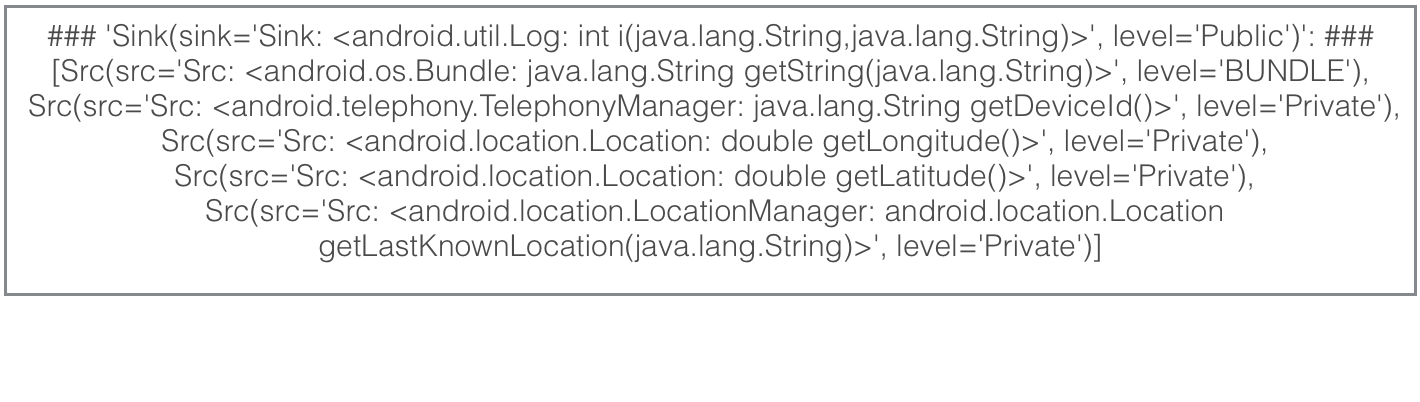
\includegraphics[scale=0.5]{Figura13}


\subsection{Asignaci�n de niveles}

Para mostrar el funcionamiento de la herramienta solo se le asigna niveles a dos categor�as como muestra la Figura 14, ya que, como se ah mencionado con anterioridad, no es necesario darle niveles a todas las categor�as participantes en los flujos de informaci�n.\par

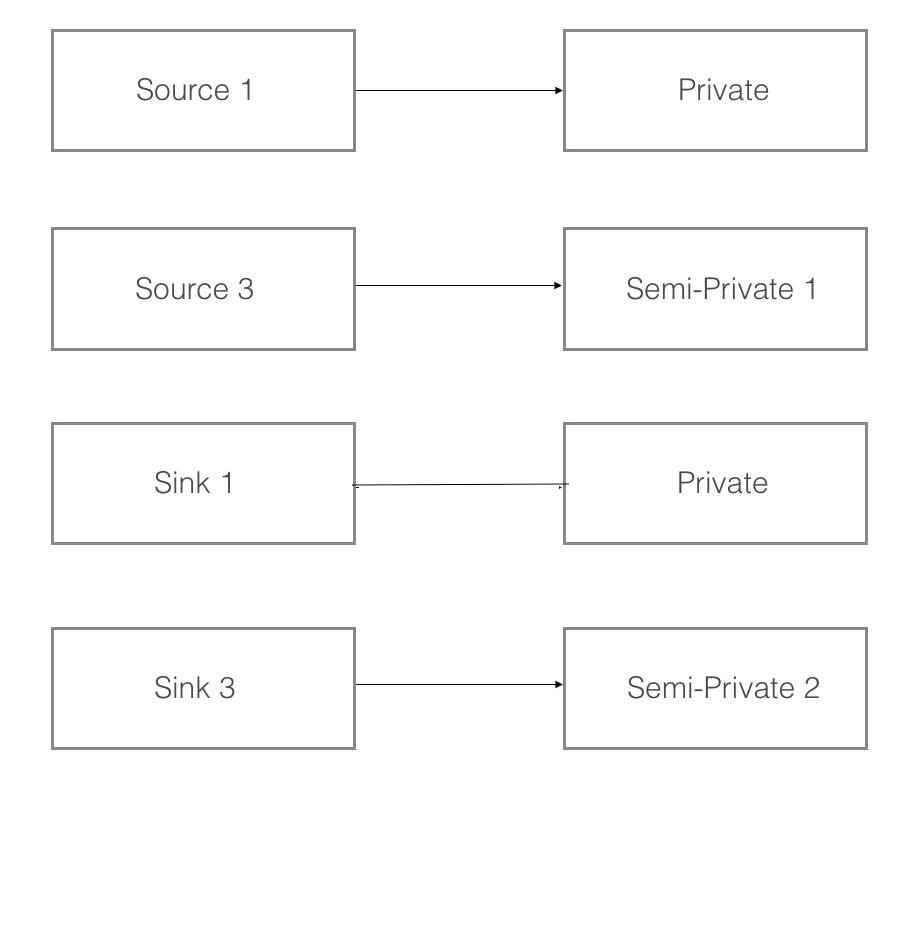
\includegraphics[scale=0.75]{Figura14}


\subsection{Excepciones}

La excepci�n de la Figura 15 hace que se ignore el flujo del device ID del usuario al Log.\par

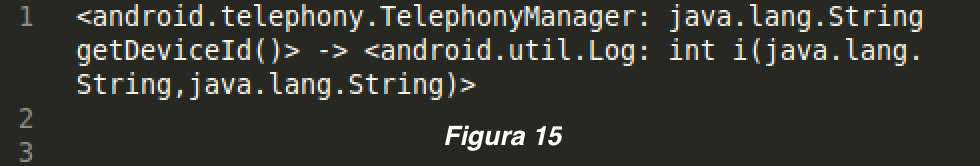
\includegraphics[scale=0.8]{Figura15}

\subsection{Didfail modificado}

La figura 16 muestra los flujos de informaci�n, los m�todos que participan y los niveles de seguridad tiene cada uno asignado.\par

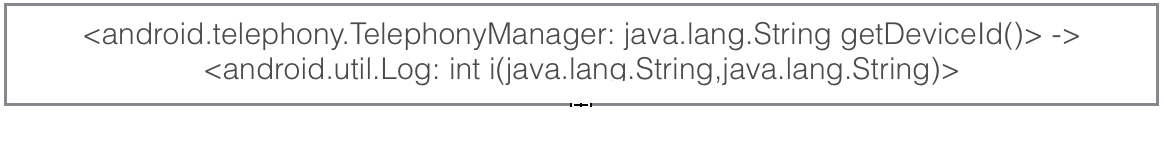
\includegraphics[scale=0.38]{Figura16}

\section{Resultados obtenidos}

Los resultados obtenidos (Figura 17) muestran que no se producen flujos de informaci�n que viole los niveles de seguridad. Ademas muestra el menor nivel posible, con respecto al orden, a cada categor�as que no ten�an nivel asignado.\par
La salida tambi�n incluye los Intent lanzados por las aplicaciones. En el conjunto actual de aplicaciones, estos ya fueron utilizados para el an�lisis y no agrega informaci�n en la salida, pero teniendo en cuenta una posible adici�n de otra aplicaci�n al conjunto, el usuario tiene la posibilidad de ver el nivel de la informaci�n que la nueva aplicaci�n puede obtener (en caso de que su manifest as� lo permita).\par

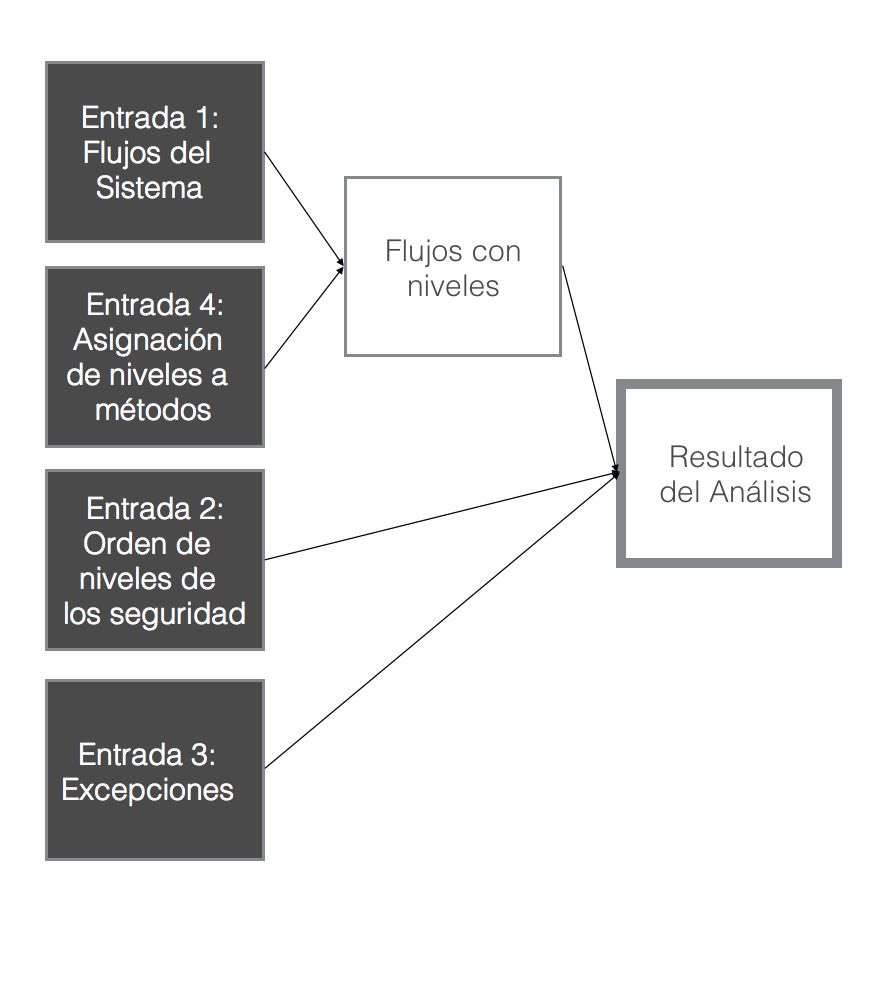
\includegraphics[scale=1]{Figura17}

El nivel asignado a la categor�a Log merece una aclaraci�n. Como se mencion� en la descripci�n de las aplicaciones a analizar, al Log le llega informaci�n desde dos lugares, el device Id del usuario con un nivel de seguridad semi-private1 y la ubicaci�n del dispositivo con nivel semi-public1. Para evitar la violaci�n de seguridad, el Log debe tener un nivel igual o mas privado que sus sources, el cual seria semi-private1 o private. Sin embargo, lo obtenido por la herramienta es semi-public1. Esto ocurre por la excepci�n dada (Figura 15), que ignora el flujo del device Id al log. 
% 
 \lhead{\emph{Conclusi�n y futuros trabajos}}

\chapter{Conclusi�n y futuros trabajos}

El an�lisis est�ticos inter e intraprocedural que lleva a cabo el prototipo descripto en este informe permite determinar el flujo de la informaci�n y esto a su vez puede ser utilizado para garantizar la confidencialidad e integridad de la informaci�n manipulada por programas Android siguiendo la configuraci�n que establezcan los usuarios de acuerdo a sus necesidades. Este prototipo tambi�n permite detectar sources y/o sinks potencialmente peligrosos y ayuda a determinar niveles de seguridad de �stos para aquellos que no tienen nivel definido por el usuario.\par
La construcci�n de este prototipo clarifica la viabilidad, eficiencia y eficacia del uso de an�lisis est�tico para la verificaci�n de confidencialidad e integridad de la informaci�n. \par
Es viable porque la implementaci�n as� lo demuestra, si bien posee muchas limitaciones y requiere refinamientos tales como la adici�n de formas en la que el flujo de informaci�n puede transmitirse, como por ejemplo los campos est�ticos, bases de datos SQLite y SharedPreferences.\par
En cuanto a la eficiencia, esto es un punto critico para los dispositivos m�viles ya que si bien cada vez son mas potentes y tiene mas recursos, el an�lisis completo requiere de un gran uso de estos y realizarlo completo en un dispositivo m�vil ser�a completamente ineficiente. Como alternativa a ello se puede dividir el an�lisis en etapas como las mencionadas en el capitulo de dise�o e implementaci�n de la herramienta, donde el repositorio de aplicaciones lleve a cabo el an�lisis mas "pesado" sobre las aplicaciones, el cual se corresponde con la etapa n�mero uno, y en el dispositivo solo se realiza la segunda etapa del an�lisis, en la cual se requiere que introduzca su configuraci�n preferida y de acuerdo a ella se complete el an�lisis. \par
Por otro lado, si bien esta herramienta requiere de refinamiento como se mencion� antes, teniendo en cuenta sus limitaciones y objetivos, realiza un an�lisis eficaz, detectando los flujos para los cuales esta capacitada para hacerlo y omitiendo aquellos en los que no se tuvieron en cuenta como por ejemplo los campos est�ticos.\par 

%% ----------------------------------------------------------------
%% ----------------------------------------------------------------

\bibliographystyle{unsrt} 
\bibliography{Biblio} 

\end{document}  
